\begin{frame}
    \frametitle{Cámara}
    
    \note{Ver libro de Sigwart. Seccion 4.2.3.2}
    \note{material sacado de mi tesis}
    \note{https://3d.bk.tudelft.nl/courses/geo1016/slides/Lecture_03_Calibration.pdf}
    
    \begin{columns}
    	\begin{column}{0.5\textwidth}
		    \begin{figure}[!h]
			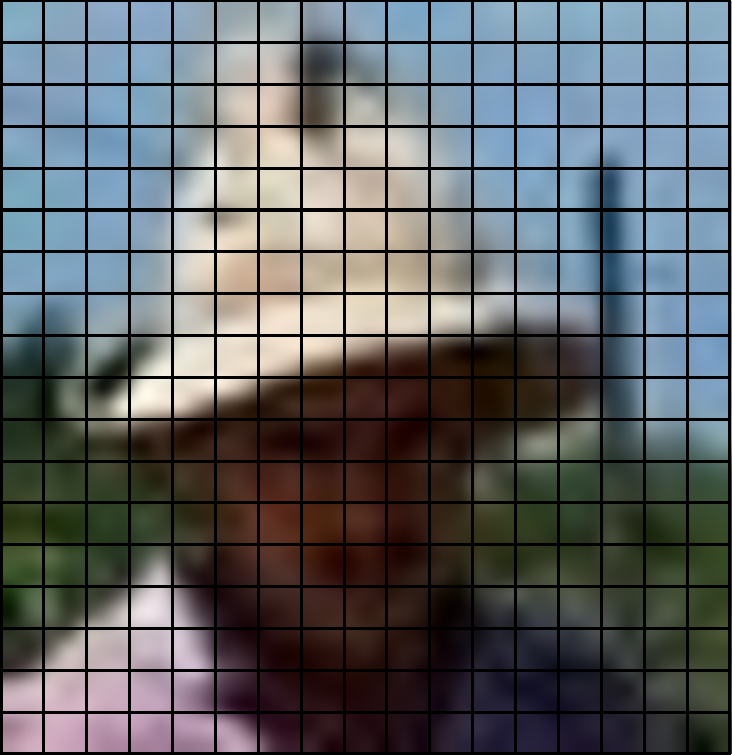
\includegraphics[width=0.6\columnwidth]{images/image_pixels.pdf}
			\end{figure}
    	\end{column}
    	\begin{column}{0.3\textwidth}
		Imagen color tiene 3 canales: R, G y B.
		\begin{equation*}
			f(x,y)=
			\begin{bmatrix}
				r(x,y) \\
				g(x,y) \\
				b(x,y)
			\end{bmatrix}
		\end{equation*}
    	\end{column}
    \end{columns}
\end{frame}

\begin{frame}
	\frametitle{Cámara}
	
%	\begin{figure}[!h]
%		\includegraphics[width=0.6\columnwidth]{images/pinhole-camera.pdf}
%	\end{figure}
\end{frame}
